\section{Theory}
\label{sec:theorie}

In the following, the theoretical basics of the diode laser are explained.

The term "laser" is an abbreviation for "light amplification by stimulated emission radiation".
Compared to other light sources, lasers have the advantage,
that they can effectively generate light with a low bandwidth in the range of $\symup{\Delta}\nu < \SI{1}{\mega\hertz}$.

The main components of the diode laser are two doped semiconductors,
one p-doped and one n-doped,
in the middle of which is an active medium.
The interfaces of the semiconductor layers are reflective,
so that an internal cavity is formed.
In order to generate a population inversion,
which is a prerequisite for the laser,
a current is passed through the three components,
as shown in \autoref{fig:aufbau_laser}.
\begin{figure}
    \centering
    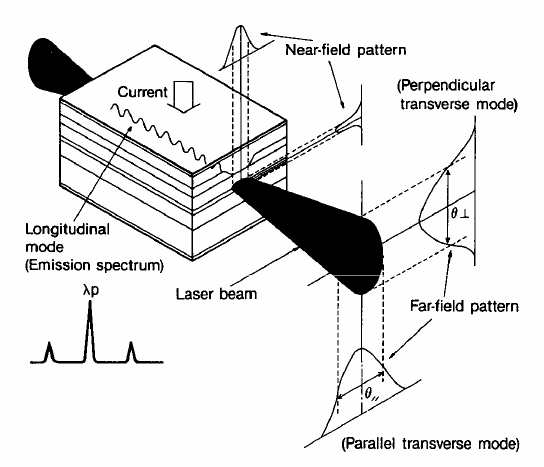
\includegraphics[width=0.7\textwidth]{content/img/p6_Fig2.png}
    \caption{General structure of a diode laser.
    An active medium is located between two differently doped semiconductors.
    If a current is sent through the diode, light is produced by emission \cite{versuchsanleitung}.}
    \label{fig:aufbau_laser}
\end{figure}
The current creates additional electron-hole pairs in the active medium.
Recombination produces photons,
which are reflected at the interfaces of the semiconductors,
forming a standing wave.
The resulting photons hit the active medium again,
so that stimulated emission occurs.
The proportion of photons,
produced by this stimulated emission of a single passing photon,
is called gain.
This only happens when a threshold current is reached.
In this case, the laser generates a coherent beam of light,
whose intensity increases linearly with the current intensity and has the form of a normal distribution.
For a current below this value, the laser behaves like an LED,
since no population inversion can be achieved.

Due to the shape of the diode, the resulting light beam is strongly divergent and is collimated with the help of a lens.
In order to achieve the smallest possible bandwidth of the wavelength,
i.e. as monochromatic a light as possible,
a diffraction grating is placed behind the diode.
A small part of the light is reflected back into the laser,
while the other part is refracted
The reflected part again provides stimulated emission,
whereby the spectrum of the resulting wavelengths is limited by the small part of the reflection.
The grating forms an external cavity together with the diode.
The addition of an optical grating to the laser diode is shown schematically in \autoref{fig:laser_system}.
\begin{figure}
    \centering
    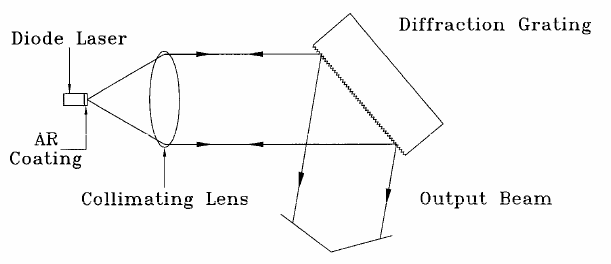
\includegraphics[width=0.9\textwidth]{content/img/p8_Fig4.png}
    \caption{Representation of the external cavity of a diode laser with an optical grating.
    A small part of the light produced in the laser is reflected by the grating, the rest is refracted.
    Taken from Ref. \cite{versuchsanleitung}.}
    \label{fig:laser_system}
\end{figure}

The resulting gain depends on the different cavities of the laser.
This is shown in \autoref{fig:gain_function}.
\begin{figure}
    \centering
    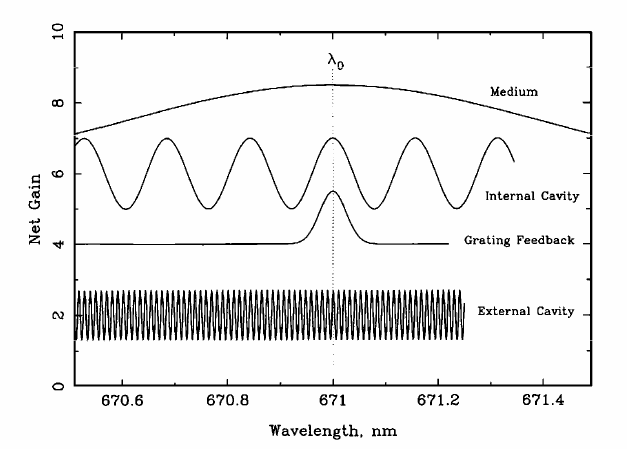
\includegraphics[width=0.7\textwidth]{content/img/p9_Fig5.png}
    \caption{Gain function depending on the different cavities of the laser.
    For the internal and external cavity,
    a standing wave results in each case,
    while the medium gain and the grating feedback show a single maximum.
    Taken from Ref. \cite{versuchsanleitung}.}
    \label{fig:gain_function}
\end{figure}
A distinction is made between the gain of the active medium,
the gain of the internal cavity and the gain of the external cavity,
as well as the grating feedback.
The maximum of the medium gain corresponds to the band gap of the active medium,
whereby a continuous spectrum results from the free mobility of the charge carriers in the bands.
The gain of the interval cavity has the form of a standing wave,
which results from the reflection of the generated light in the resonator.
The period of this standing wave,
also called the "free spectral range",
can be determined using the equation $\symup{\Delta}\nu_\text{FSR} = \sfrac{c}{2Ln}$,
where $L$ is the length of the cavity and $n$ is the refractive index.
For the grating feedback, there is a single narrow maximum,
which corresponds to the wavelengths of the light reflected back to the laser.
All other wavelengths are scattered by the grating.
For the gain of the external cavity, the same results as for the internal cavity,
due to the reflection of light between the optical grating and the laser diode.
In this case the period is described by $\symup{\Delta}\nu_\text{FSR} = \sfrac{c}{2L}$.
The final wavelength of the laser can be determined using the equation $\lambda = d \cdot \sin{(\theta)}$,
where $d$ is the line number of the grating,
and $\theta$ is the grating angle.
The superposition of the gain of the external cavity and the grating feedback is considered.

Both the medium gain,
as well as that of the internal cavity depend on the current and thus on the temperature of the diode,
because the diode heats up when the current increases.
In this way, the concentration of the charge carriers in the active medium also changes.
The wavelength of the resulting radiation increases linearly with the current intensity and the temperature.
However, the wavelengths of the different components change differently with changes in the current,
so that so-called mode hops occur,
which are exemplified in \autoref{fig:modehops},
where in this case the grating angle was varied.
\begin{figure}
    \centering
    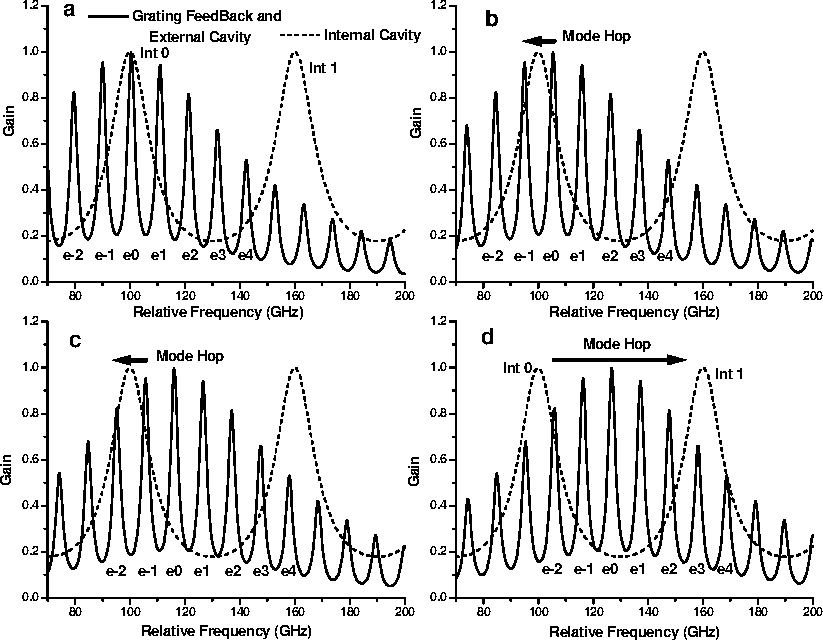
\includegraphics[width=0.7\textwidth]{content/img/p13_Fig9.pdf}
    \caption{Representation of mode hops in the gain of the external cavity and the grating feedback with variation of the grating angle \cite{versuchsanleitung}.}
    \label{fig:modehops}
\end{figure}
